% !TEX root = ../../../MathModel.tex
% 负责人：罗财能。
% 给出运输与中继联合方案，检查货箱交付、资源占用和全过程通信保障。
% 联合任务完成时间涵盖两类无人机返航；将完整方案交接给问题四。
\subsubsection{模型求解}
\label{sec:q3:solution}

\textbf{求解流程与评价顺序。}
采用“多起点构造、固定结构排程改进、独立复核”的求解流程。
首先在离散中继候选点上，改变组批偏好、紧迫度规则及等待与能耗权重，
运行36组构造搜索；候选运输架次最多访问3个服务区，并以固定随机种子
20260924记录扰动过程。题目未指定多个评价指标的优先级，本文选择依次比较
加权配送延迟、联合完成时间、总能耗和两类总架次数的字典序，
将医疗与首批保障期限作为必须满足的约束，而不以罚函数替代。

随后选取3个代表性任务结构，固定货箱组批、访问顺序、运输机型、
中继位置及保障关联，使用CP-SAT重新安排开始时刻与实体资源。
每个结构分配60\,s预算，先用30\,s降低加权延迟，再以不增加该阶段所得延迟为条件，
用30\,s缩短联合完成时间；总预算180\,s并非实际必然耗时。
排程采用1\,s网格，对占用时长向上取整、硬期限向下取整，
并将中继服务结束时间延长2\,s以容纳取整误差，附加悬停能耗重新计入。
三个结构均使用单工作线程，随机种子依次为20260924、20260925和20260926。
最终选中第二个改进方案，其两阶段求解状态均为\texttt{FEASIBLE}；
第三个结构虽取得限定排程模型内的\texttt{OPTIMAL}状态，评价仍劣于所选方案。
因此，以下结果是限定候选搜索得到的可行方案，不是原问题的全局最优解。

\textbf{运输效果与指标权衡。}
独立重算得到表\ref{tab:q3:overall}的结果。
80箱物资全部且仅交付一次，其中医疗物资与首批保障货箱的并集为31箱，均满足硬期限。
其余物资中6箱晚于期望时间，分别涉及S001的3箱饮用水、S006的1箱饮用水，
以及S002、S013各1箱食品；最长延迟为1246.434\,s，即20.77\,min。
图\ref{fig:q3:delivery}显示交付进度及逐箱期望时限的比较；
图中的期望时刻不替代逐箱硬截止时刻的核验。

\begin{table}[htbp]
  \centering
  \caption{联合调度方案的主要指标}
  \label{tab:q3:overall}
  \begin{tabular}{lr}
    \toprule
    指标 & 数值 \\
    \midrule
    已交付货箱数／硬时限违约箱数 & 80／0 \\
    运输架次数／中继架次数 & 33／8 \\
    最后一箱交付时刻（min） & 145.75 \\
    运输全部返航时刻（min） & 154.15 \\
    联合全部返航时刻（min） & 161.37 \\
    运输能耗／中继能耗（kWh） & 76.682／4.004 \\
    联合总能耗（kWh） & 80.686 \\
    加权延迟 $W$（s） & 37597.854 \\
    普通物资延迟箱数／最长延迟（min） & 6／20.77 \\
    运输／中继最低返航SOC（\%） & 21.49／62.88 \\
    \bottomrule
  \end{tabular}
\end{table}

与所选结构改进前的排程相比，加权延迟由182621.303\,s降至37597.854\,s，
减少79.41\%，而联合完成时间由156.73\,min增至161.37\,min。
这反映了延迟优先的取舍，不能据此声称所有指标同时改善。
尽管候选集包含多点架次，最终所选33个运输架次均为单服务区往返；
该结果说明当前资源与时限下此构造更有利于所采用的评价顺序，
不构成单点往返优于所有多点方案的普遍结论。

\begin{figure}[htbp]
  \centering
  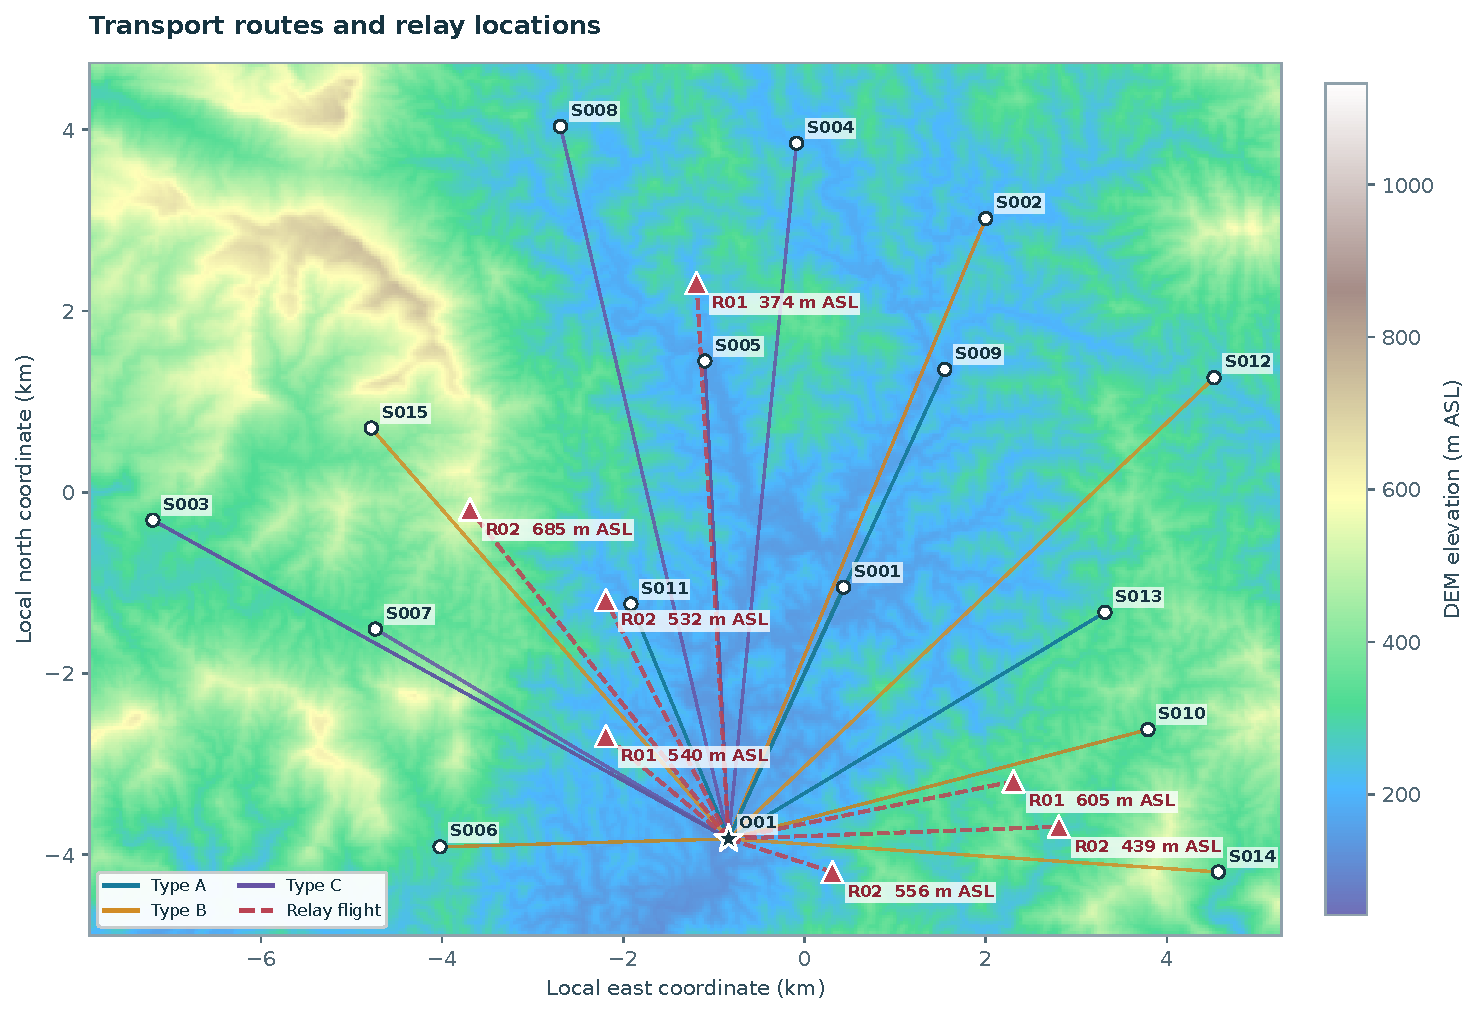
\includegraphics[width=0.96\textwidth,height=0.60\textheight,keepaspectratio]
    {../Results/Q3/01_routes_and_relays.pdf}
  \caption{运输航路与中继悬停位置；同一中继机可在不同时段使用不同位置}
  \label{fig:q3:routes}
\end{figure}

\textbf{中继与资源周转安排。}
图\ref{fig:q3:routes}展示最终航路及7个不同中继位置，
8个中继架次的主要时序见表\ref{tab:q3:relay-schedule}。
服务开始时刻均为建链完成时刻，海拔采用绝对高程；
对应悬停离地高度为150\,m或300\,m，均不超过上限。
R006承担较长的通信服务，最终于161.37\,min返航，
因此联合完成时间比运输全部返航时间晚7.22\,min。

\begin{table}[htbp]
  \centering
  \caption{中继架次的位置与服务时序}
  \label{tab:q3:relay-schedule}
  \small
  \setlength{\tabcolsep}{3pt}
  \resizebox{\textwidth}{!}{%
  \begin{tabular}{llrrrcrr}
    \toprule
    架次 & 执行机 & 经度（$^\circ$） & 纬度（$^\circ$） & 海拔（m） & 服务时段（min） & 返航（min） & 能耗（kWh） \\
    \midrule
    R001 & R01 & 109.261550 & 23.014239 & 604.9 & 12.39--25.82 & 32.04 & 0.435 \\
    R002 & R02 & 109.266428 & 23.009725 & 439.4 & 48.64--59.12 & 64.92 & 0.385 \\
    R003 & R02 & 109.217643 & 23.032299 & 532.2 & 13.58--29.24 & 34.78 & 0.458 \\
    R004 & R01 & 109.217643 & 23.018754 & 540.3 & 82.81--97.09 & 101.35 & 0.383 \\
    R005 & R01 & 109.227400 & 23.063903 & 374.3 & 48.41--62.42 & 70.62 & 0.550 \\
    R006 & R02 & 109.203007 & 23.041329 & 685.3 & 102.29--153.14 & 161.37 & 1.188 \\
    R007 & R01 & 109.217643 & 23.032299 & 532.2 & 115.66--127.97 & 133.51 & 0.397 \\
    R008 & R02 & 109.242036 & 23.005210 & 556.0 & 76.55--82.61 & 86.32 & 0.209 \\
    \bottomrule
  \end{tabular}}
\end{table}

表\ref{tab:q3:transport-use}按机型汇总运输任务。
实际使用8架运输机及13组运输电池，另使用2架中继机和4组能源组件。
图\ref{fig:q3:resources}将实体机占用与能源资源充电分开记录，
同一能源资源再次使用前均已满电，且中继机返航后的周转时间得到保留。
最低运输返航SOC为21.49\%，高于20\%下限约1.49个百分点，
说明部分运输任务的能量余量较紧；中继最低SOC为62.88\%，
但较多剩余能量并不意味着中继位置、服务时段和实体机冲突可以忽略。

\begin{table}[htbp]
  \centering
  \caption{运输机型任务与能源资源使用汇总}
  \label{tab:q3:transport-use}
  \begin{tabular}{lrrrrr}
    \toprule
    机型 & 架次数 & 交付箱数 & 实体机数 & 电池组数 & 能耗（kWh） \\
    \midrule
    A & 18 & 31 & 4 & 6 & 29.050 \\
    B & 9 & 20 & 2 & 4 & 17.074 \\
    C & 6 & 29 & 2 & 3 & 30.558 \\
    合计 & 33 & 80 & 8 & 13 & 76.682 \\
    \bottomrule
  \end{tabular}
\end{table}

\begin{figure}[htbp]
  \centering
  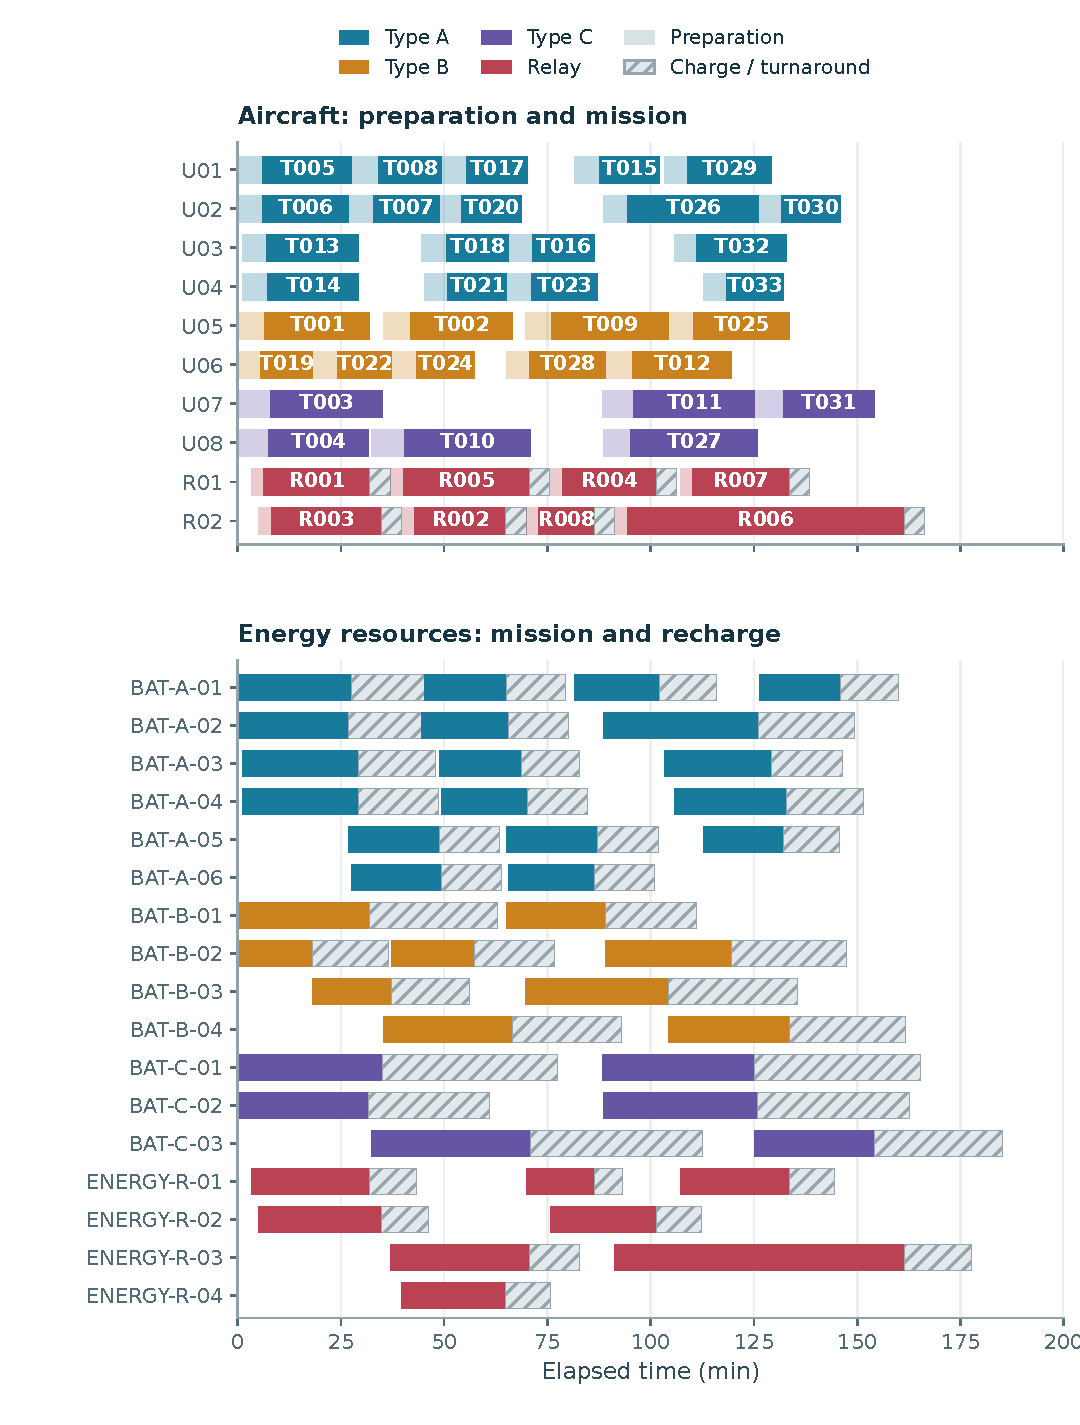
\includegraphics[width=0.98\textwidth,height=0.86\textheight,keepaspectratio]
    {figures/problem3/resource_schedule.pdf}
  \caption{实体无人机与能源资源占用；灰色斜线表示充电或中继机周转}
  \label{fig:q3:resources}
\end{figure}

\begin{figure}[htbp]
  \centering
  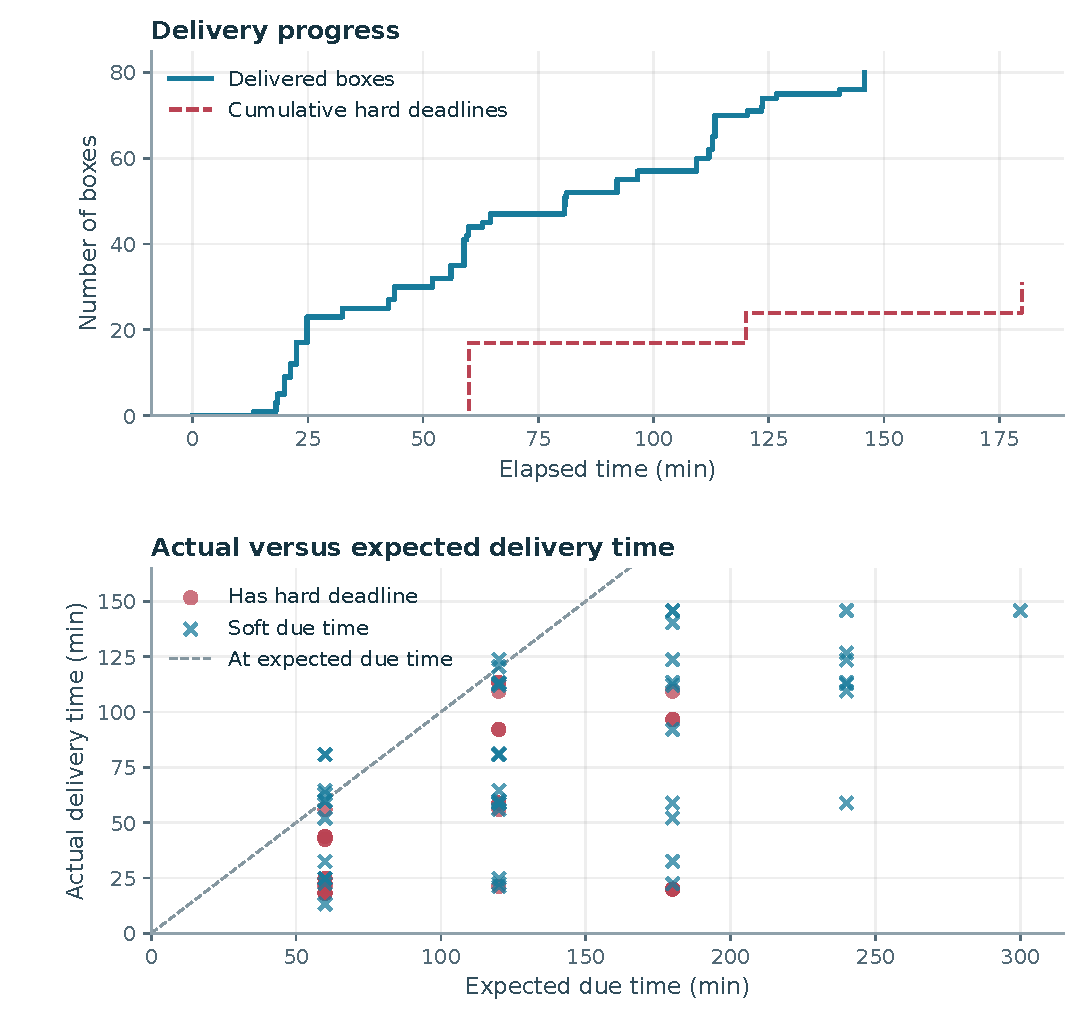
\includegraphics[width=0.98\textwidth,height=0.74\textheight,keepaspectratio]
    {figures/problem3/delivery_performance.pdf}
  \caption{累计交付进度及实际交付时刻与期望时限的比较}
  \label{fig:q3:delivery}
\end{figure}

\textbf{通信核验与结果交接。}
以2\,s步长独立检查20479个通信样本，按直连优先规则得到14131个直连样本、
6348个中继样本和0个中断样本。有限采样本身不能证明连续通信，
程序另对4208个时间区间验证保守链路裕量下界，全部通过，
从而在原始DEM分片常高像元模型内认证全过程通信。
通信结果表记载的是区间保底保障预约，不能直接解释为实际状态的持续时间；
即使已有中继预约，网关直连可用时仍记为直连。

完整组批、路线、逐箱时刻、中继关联与资源编号保存在
\path{Group/Lcn/Results/Q3/solution.json}及配套CSV中，
独立复核文件\texttt{validation.json}记录零错误，可供问题四冻结并继承。
结论受离散中继候选、有限路线搜索、补充能耗公式及并行工位和充电假设限制；
尚未计入未给定的天气扰动、无线干扰及亚像元地形，不将模型可行性等同于实地保障率。

\clearpage
